\chapter{Metodología}
\label{chap:metodologia}

\section{Diagnóstico de la Situación Actual}

El punto de partida del proyecto es una máquina dosificadora de granos de arquitectura electromecánica heredada, que opera como una ``caja negra'' en el Laboratorio de Procesos de la Universidad Indoamérica. Su funcionamiento original se basa en un circuito de potencia a 220 V controlado por un PLC sin interfaces de red ni telemetría. El ciclo de dosificación se inicia al recibir una señal en la entrada 1 del PLC, proveniente del contactor trifásico del motor principal. A partir de esa señal, el PLC activa relés secuenciales que gobiernan electroválvulas y pistones de dos estados, sin posibilidad de modificar su lógica interna ni su cableado, por políticas institucionales que impedían la manipulación completa de la máquina.

Para caracterizar este funcionamiento se aplicaron técnicas de ingeniería inversa, empleando multímetros y trazados de continuidad para mapear las rutas de energía y la secuencia de activación de los actuadores. La observación directa estructurada permitió identificar los tiempos de ciclo, las condiciones de enclavamiento y la ausencia total de monitoreo en tiempo real, lo que confinaba el mantenimiento a un enfoque exclusivamente reactivo. Este esquema de operación contrasta con las demandas de los entornos de producción inteligente, que exigen visibilidad continua de las variables de proceso para la toma de decisiones basada en datos \cite{retrofitting2025}.

Las limitaciones más críticas detectadas fueron: (1) la imposibilidad de modificar el cableado interno, (2) la falta de registro de estados discretos y (3) la nula visibilidad de las variables de proceso. Ante estas restricciones se diseñó una integración ciberfísica mediante un \textit{bypass} no intrusivo, que bifurca las rutas de energía hacia un banco de relés independientes comandado por un microcontrolador ESP32. Esta intervención garantiza la operación dual: si el nodo IoT falla, el PLC legacy mantiene su funcionalidad original, preservando la integridad del equipo. La estrategia se complementó con la instrumentación de sensores infrarrojos, un sensor ultrasónico y un transductor de presión industrial, todos aislados galvánicamente mediante optoacopladores PC817. La solución representa una modernización \textit{retrofit} en la capa de control, respetando el principio de no intromisión sobre la lógica original del PLC, en línea con las recomendaciones de la ISO 23247-1 para gemelos digitales que deben coexistir con equipamiento heredado \cite{iso23247-1}.

\begin{figure}[htbp]
\centering
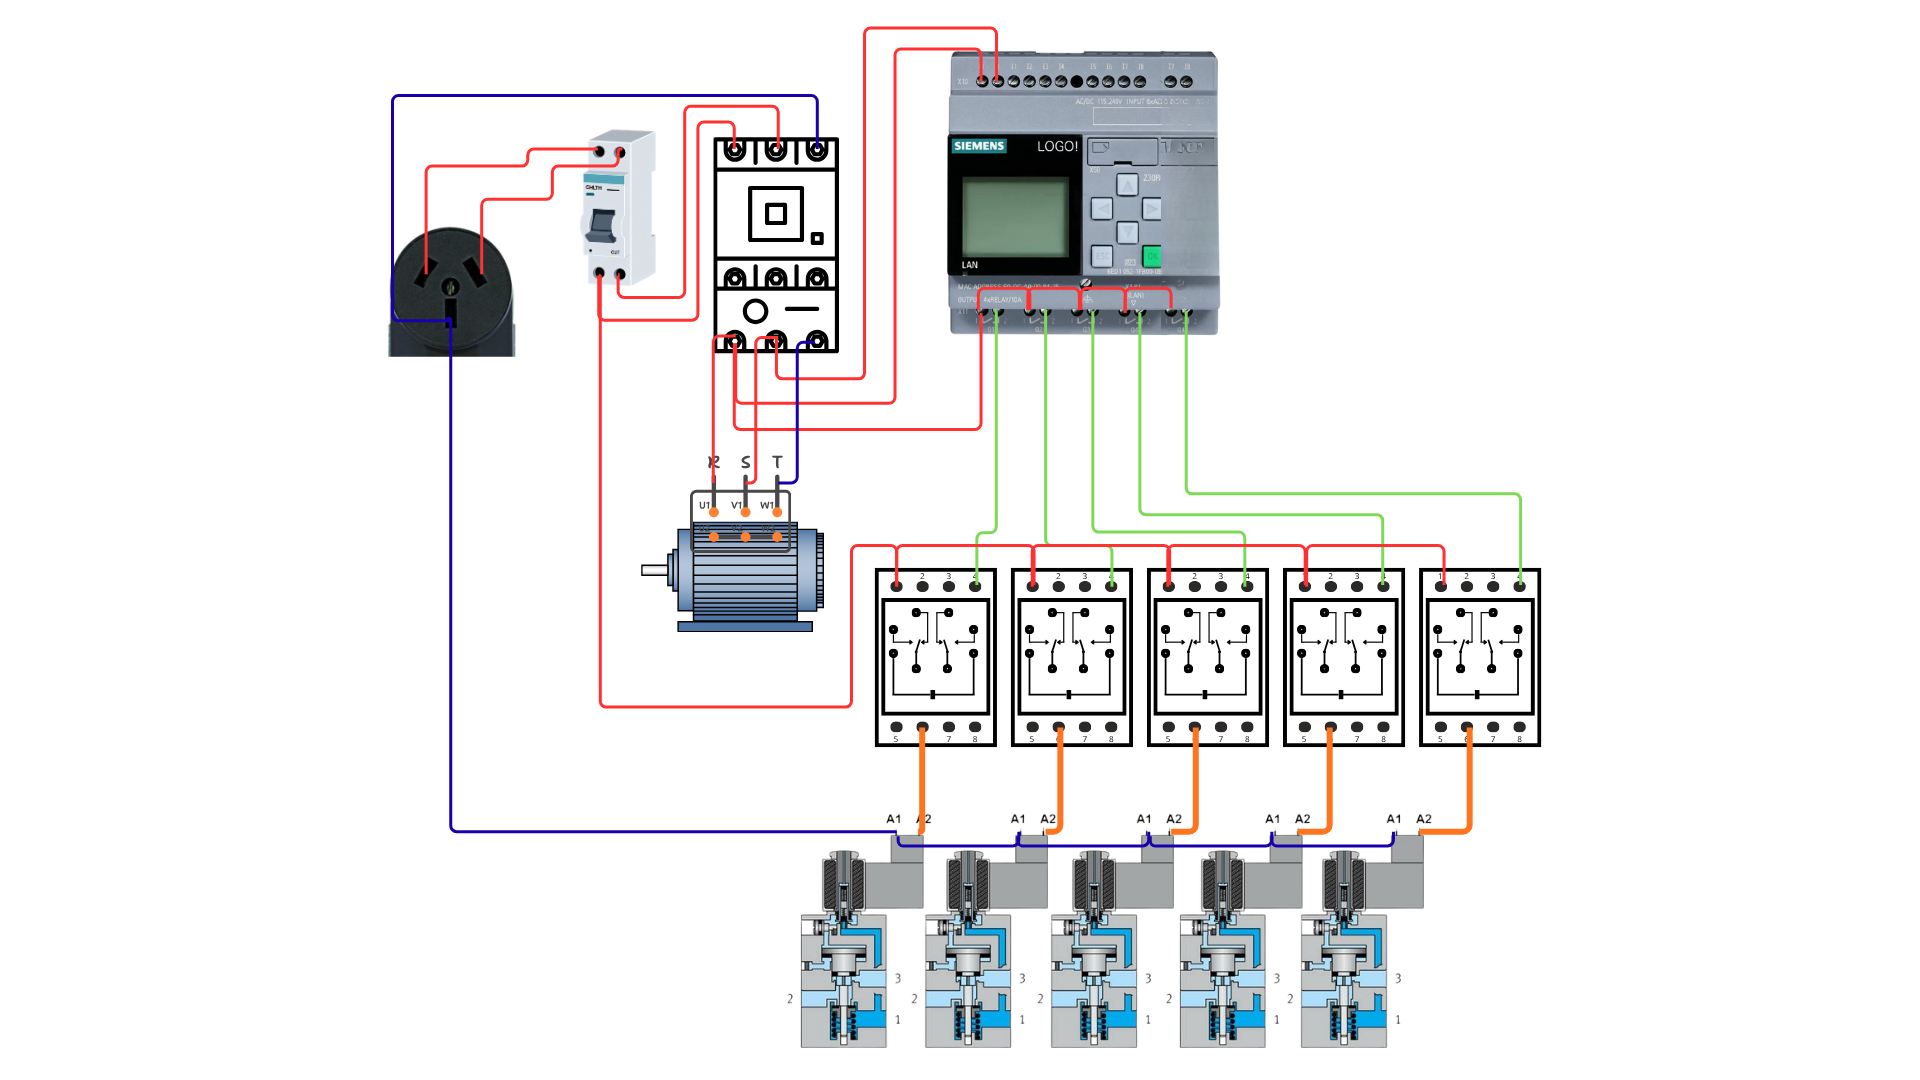
\includegraphics[width=0.80\textwidth]{Capítulos/fig/mapeo_señales.png}
\caption{Mapeo de señales originales, puntos de intervención y arquitectura de bypass.}
\label{fig:diag_diag}
\end{figure}

\section{Metodología de Desarrollo e Implementación}

Con el objetivo de alinear cada fase de diseño con su correspondiente validación técnica, se adoptó el modelo en V (\textit{V-Model}) adaptado a sistemas ciberfísicos. Esta metodología mitiga los riesgos de asincronía entre el modelo físico y su réplica virtual, garantizando que los requisitos sean verificados incrementalmente.

Las fases de ingeniería se estructuraron de la siguiente manera:

\begin{enumerate}
    \item \textbf{Fase 1 – Definición Arquitectónica.} Levantamiento del diagrama de estados original y definición de las capas ciberfísicas conforme a la familia de estándares ISO 23247 para gemelos digitales en manufactura. Se identificaron los flujos de información necesarios para el gemelo digital de nivel 3 (predictivo/interactivo), según la clasificación de madurez que establece la parte 2 de dicha norma \cite{iso23247-2}.
    
    \item \textbf{Fase 2 – Diseño de Subsistemas.} Modelado cinemático en Webots, programación de la máquina de estados finitos (FSM) en Python, diseño del SCADA en Node-RED y definición de los tópicos MQTT bajo el protocolo de mensajería ligera estandarizado por OASIS \cite{oasis2014}.
    
    \item \textbf{Fase 3 – Implementación Física.} Construcción del panel de control con grado de protección IP54, soldadura de la instrumentación aislada con optoacopladores, despliegue del broker Mosquitto y grabación del firmware en los dos microcontroladores ESP32.
    
    \item \textbf{Fase 4 – Verificación (Virtual Commissioning).} Ejecución de la FSM en Webots con inyección de perturbaciones y sincronización con los tópicos MQTT, utilizando la máscara de enrutamiento de Node-RED para aislar los comandos del hardware.
    
    \item \textbf{Fase 5 – Validación del Sistema.} Extracción de logs para el cálculo de latencias de red, tiempos de recuperación y la métrica de efectividad mecánica operativa (EMO) adaptada del OEE, conforme a los lineamientos de indicadores clave de desempeño de la ISO 22400 \cite{iso22400-2}.
\end{enumerate}

\begin{figure}[htbp]
\centering
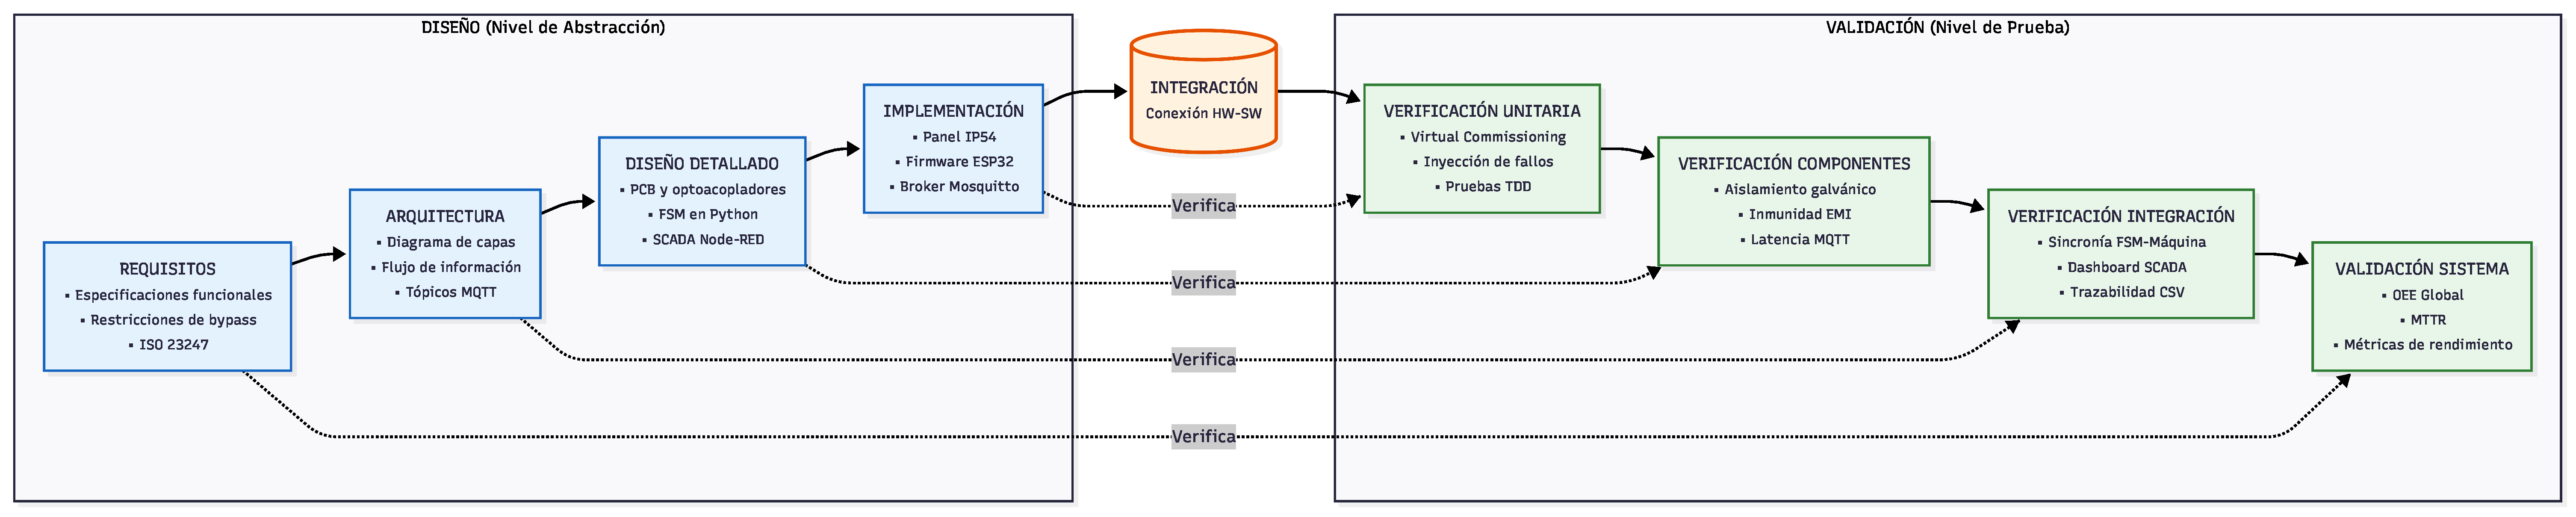
\includegraphics[width=0.9\textwidth, height=0.3\textheight, keepaspectratio=false]{Capítulos/img/V-MODEL.pdf}
\caption{Metodología V-Model aplicada al desarrollo del gemelo digital.}
\label{fig:diag_vmodel}
\end{figure}

\section{Técnicas e Instrumentos de Recolección de Información}

\subsection{Técnicas de Diagnóstico Físico}

La caracterización de la máquina legacy se sustentó en observación directa estructurada de los ciclos de dosificación y en el análisis de las señales eléctricas mediante un multímetro. Se realizó un mapeo completo de la secuencia electroneumática, registrando los tiempos de activación de las electroválvulas y el desplazamiento de los pistones con resolución de milisegundos. El uso de trazados de continuidad permitió identificar los puntos de bifurcación para el bypass sin alterar el cableado original, una práctica común en proyectos de retrofitting de maquinaria industrial \cite{retrofitting2025}.

\subsection{Instrumentos de Validación del Gemelo Digital}

El controlador de la FSM ejecutado en el entorno Webots genera un registro automático de transiciones de estado en archivos CSV con marcas de tiempo precisas. Durante las pruebas se almacenan, además de los cambios de estado, las latencias cinemáticas entre la orden enviada y la respuesta del actuador virtual. Estos datos constituyen la base para el cálculo posterior de la métrica EMO.

\subsection{Recolección de Telemetría MQTT}

La arquitectura de comunicación se fundamenta en una jerarquía estricta de tópicos. Los nodos ESP32 publican periódicamente las lecturas de los sensores bajo \texttt{maquina/sensor/\#} y los comandos de actuación fluyen por \texttt{maquina/actuador/\#}. Cada mensaje contiene un payload en formato JSON con los campos \texttt{timestamp}, \texttt{valor}, \texttt{unidad} y \texttt{calidad}. La frecuencia de muestreo se fijó en 100 ms para asegurar un sincronismo adecuado entre la planta física y el SCADA, aprovechando las características de baja latencia del protocolo MQTT \cite{oasis2014}.

\begin{figure}[htbp]
    \centering
%    \begin{minipage}{0.48\textwidth}
    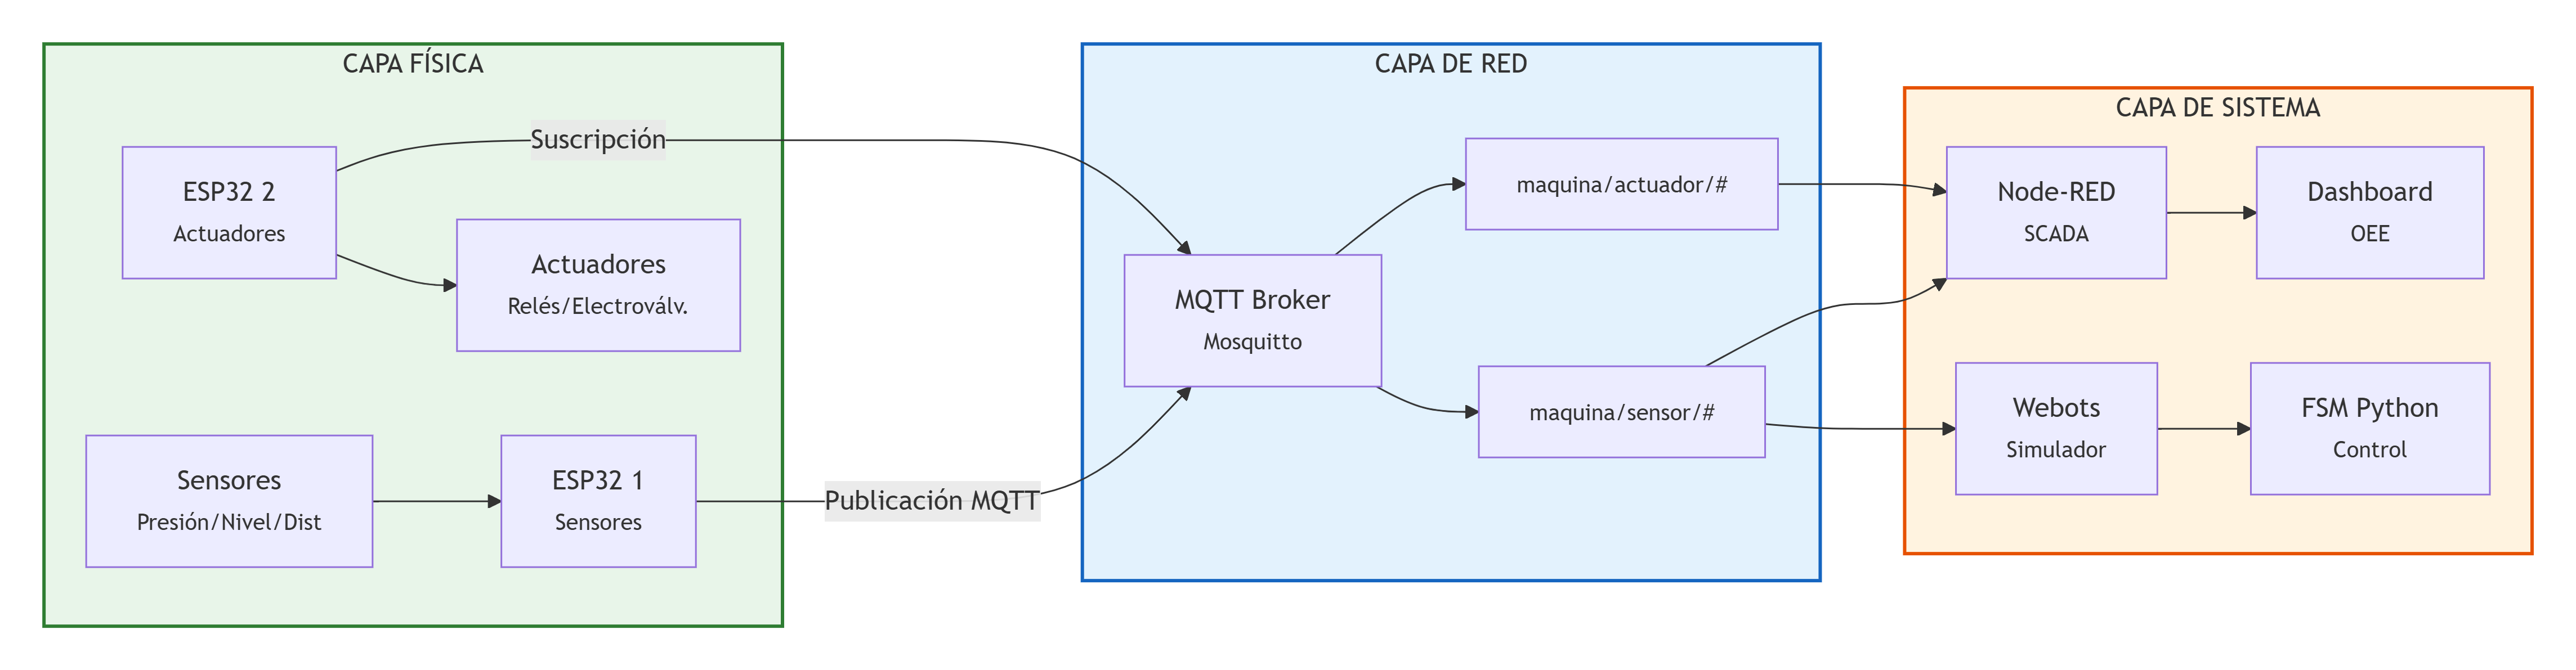
\includegraphics[width=0.9\textwidth, height=0.1\textheight, keepaspectratio=false]
    {Capítulos/img/flujomqtt.png}
    
\caption{Flujo completo de datos, formatos de payload y frecuencias de publicación.}
\label{fig:diag_flujo_info}
%\end{minipage}
\end{figure}

\section{Configuración e Implementación de Equipos}

\subsection{Configuración del ESP32 como Nodo de Borde}

Los dos microcontroladores ESP32-DevKit v1 (38 pines) fueron configurados con las siguientes asignaciones de pines:
\begin{itemize}
    \item Sensores infrarrojos (entrada digital con optoacoplador PC817) en GPIO 14, 15, 16.
    \item Sensor ultrasónico HC-SR04: Trig en GPIO 17, Echo en GPIO 18.
    \item Transductor de presión industrial 4-20 mA, leído a través de un conversor analógico-digital con filtro de promedio móvil de 10 muestras.
    \item Display TM1637 (I2C) y expansores de puertos PCF8574 para la interfaz HMI física.
    \item Cliente MQTT implementado con la librería \texttt{PubSubClient}; conexión WiFi con QoS 1 para los tópicos de estado y comandos.
\end{itemize}

Se implementaron filtros digitales de promedio móvil para suavizar las lecturas analógicas de presión y eliminar el ruido de alta frecuencia inducido por el contactor trifásico. La plataforma ESP32 fue seleccionada por su conectividad WiFi integrada, su arquitectura de doble núcleo que permite ejecutar simultáneamente la pila de comunicación MQTT y la lógica de control, y un costo reducido que la convierte en una opción idónea para nodos de borde en entornos IIoT \cite{espressif2023}.

\subsection{Configuración del Broker Mosquitto}

El broker MQTT se desplegó sobre un sistema operativo Linux en una máquina virtual dedicada. Se habilitaron los puertos 1883 (MQTT) y 9001 (WebSockets), y se aplicó autenticación básica (usuario/contraseña) para restringir accesos no autorizados. Se activó la persistencia de mensajes y la retención de estados (\textit{retained messages}) para que los suscriptores nuevos reciban de inmediato el último valor conocido de cada sensor, garantizando la consistencia del estado incluso después de desconexiones temporales.

\subsection{Configuración de Node-RED como SCADA}

Se instalaron los nodos adicionales para MQTT (entrada/salida), \texttt{Dashboard}, \texttt{JSON parser} y \texttt{SQLite}. Los flujos principales son:
\begin{itemize}
    \item Suscripción a los tópicos \texttt{maquina/sensor/\#} para visualización en tiempo real.
    \item Enrutamiento condicional: cuando el selector físico está en modo \textit{Simulación}, los comandos de actuador se publican bajo el prefijo \texttt{maquina/simulacion/actuador/\#}, que es leído exclusivamente por el controlador de Webots, aislándolo del hardware.
    \item Almacenamiento de los datos históricos en una base SQLite para el análisis post-prueba.
\end{itemize}

La elección de Node-RED responde a su modelo de programación visual, su conectividad nativa con MQTT y la capacidad de generar dashboards web de manera ágil, cualidades que han sido validadas en numerosos casos de uso de la Internet de las Cosas.

\subsection{Configuración de Webots como Simulador Ciberfísico}

Los modelos 3D generados en FreeCAD se importaron en formatos STL y OBJ. Los pistones se modelaron mediante nodos \texttt{SliderJoint} con dos posiciones discretas, y las trampillas con nodos \texttt{HingeJoint}. El controlador Supervisor, escrito en Python, ejecuta la FSM y utiliza el cliente Paho-MQTT para suscribirse y publicar en los tópicos correspondientes. La sincronización se logra a través de un lazo de control que, cada 100 ms, envía el estado actual del gemelo a \texttt{maquina/estado/fsm}.

Webots fue seleccionado por superar a otros simuladores en los criterios de integración con Python, bajo consumo de CPU y capacidad para modelar restricciones mecánicas discretas sin necesidad de motores físicos complejos \cite{michel2004}. La simulación no exige recursos de GPU elevados, lo que permite ejecutarla en el mismo equipo que aloja el SCADA y el broker MQTT durante las pruebas de laboratorio.

\begin{figure}[htbp]
\centering
    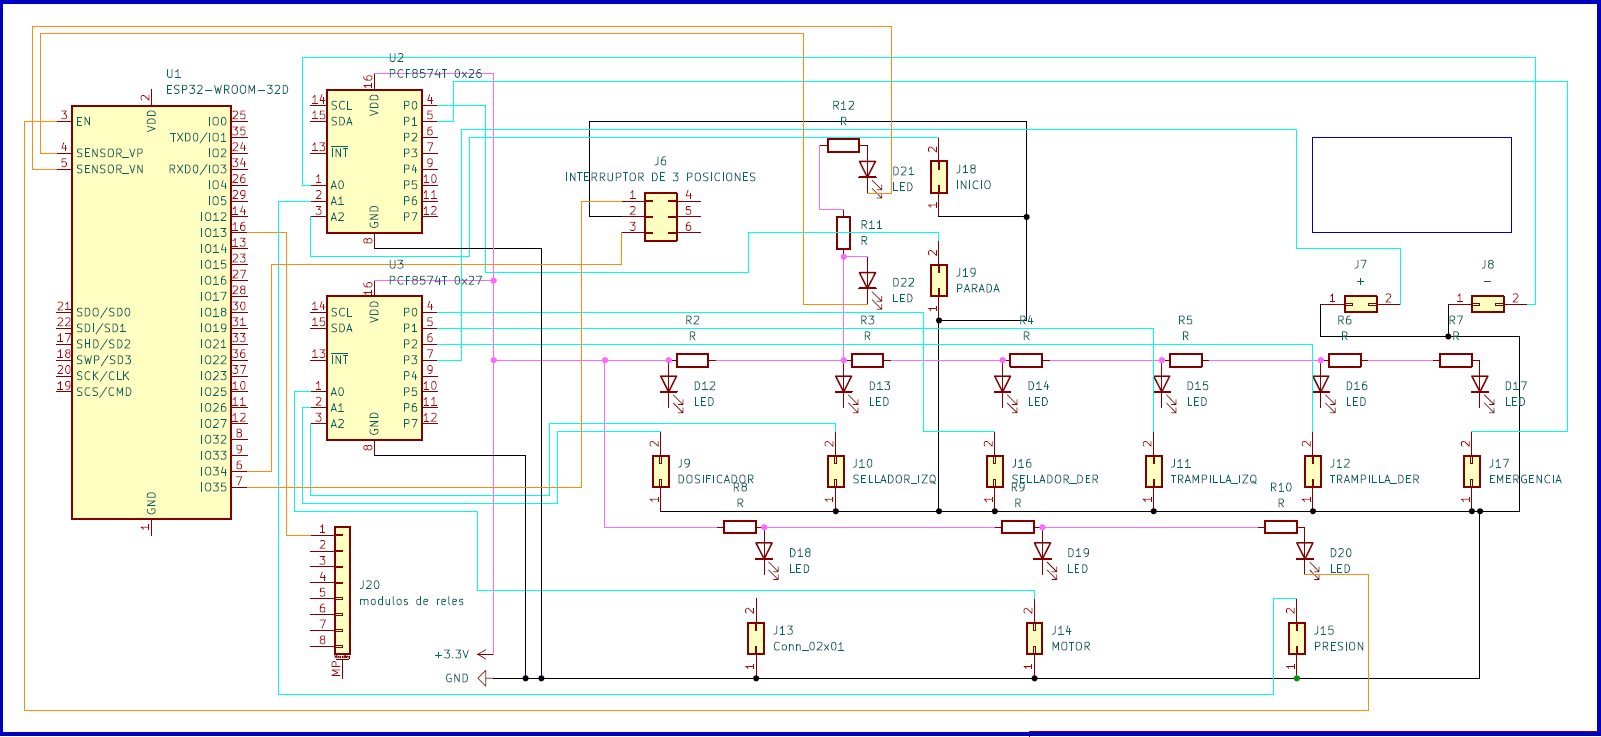
\includegraphics[width=1\textwidth]{Capítulos/img/DIAGRAMA ESQUEMATICODELPANELSCADA.png}
\caption{Esquemático del panel de control IP54.}
\label{fig:esq_panel}
\end{figure}

\begin{figure}[htbp]
\centering
    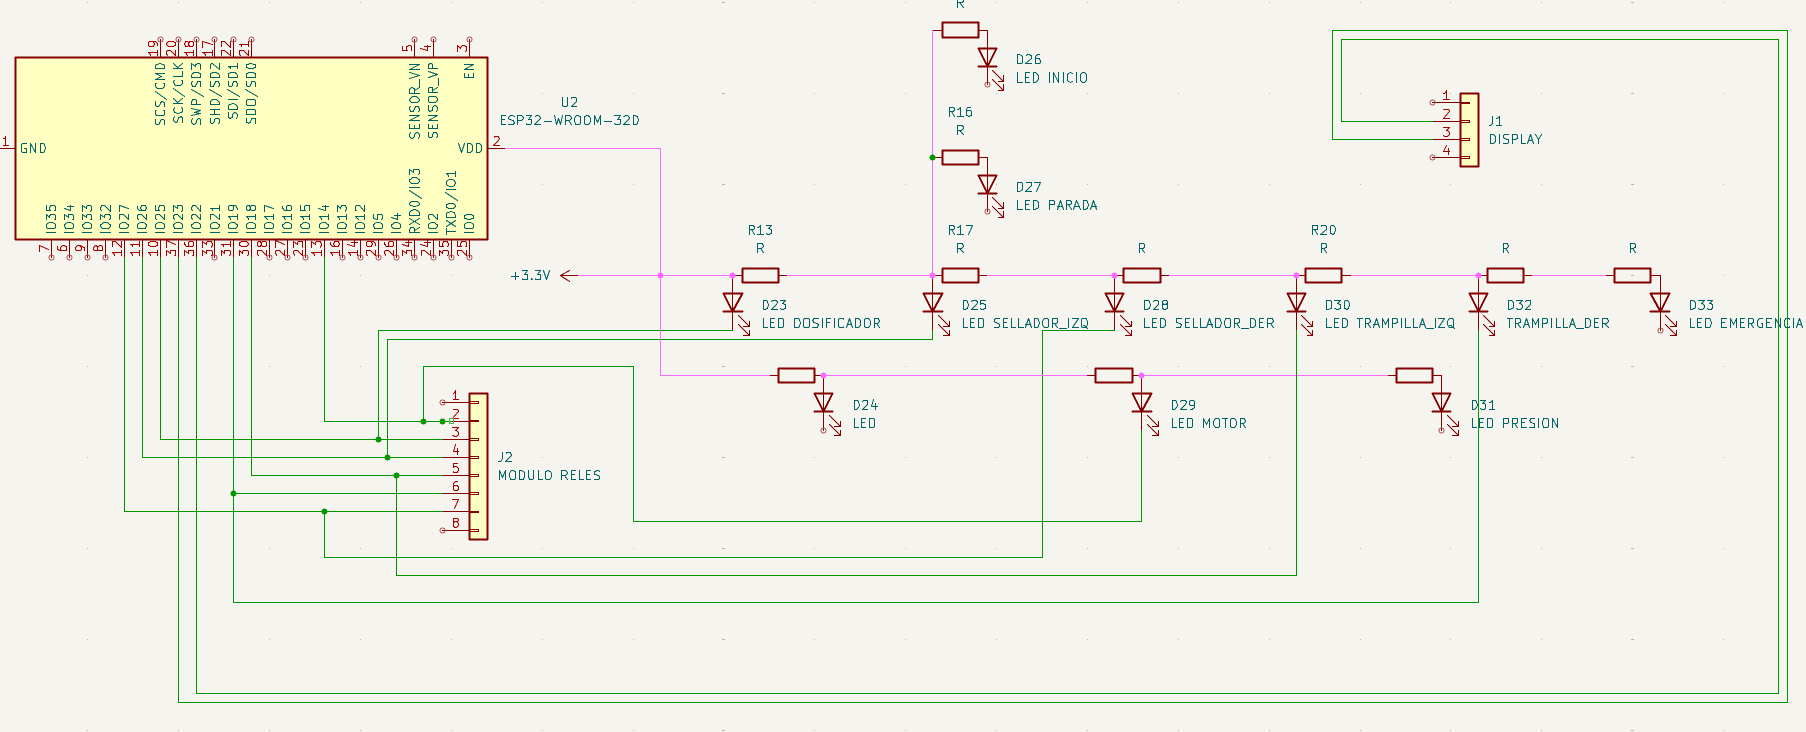
\includegraphics[width=1\textwidth]{Capítulos/img/DIAGRAMARELES.png}
\caption{Conexión de relés.}
\label{fig:conex_relays}
\end{figure}

\section{Requerimientos del Sistema}

\subsection{Requerimientos Funcionales}

\begin{enumerate}
    \item \textbf{RF1 – Control Híbrido y Bypass.} El panel físico instrumentado debe permitir la alternancia entre modo Manual (control unitario) y modo Automático, aislando estas rutinas de la lógica original del PLC mediante el banco de relés independientes.
    \item \textbf{RF2 – Enclavamiento de Seguridad (Interlocks).} El algoritmo de la FSM debe impedir la activación manual de cualquier actuador mientras el ciclo automático esté en ejecución.
    \item \textbf{RF3 – Fidelidad Cinemática en 3D.} El gemelo digital, desarrollado en Webots, debe emular los pistones neumáticos respetando exactamente sus dos posiciones discretas y las restricciones mecánicas de la máquina real.
    \item \textbf{RF4 – Secuestro de Señales (Aislamiento Virtual).} Node-RED debe interceptar las órdenes de control e inyectar el prefijo de simulación (e.g., \texttt{maquina/simulacion/actuador/piston}) cuando el selector de modo esté en Simulación, comandando únicamente al gemelo sin accionar el hardware físico.
    \item \textbf{RF5 – Telemetría en Tiempo Real.} El ESP32 debe publicar lecturas de los sensores cada 100 ms en los tópicos MQTT, indicando marca temporal y calidad del dato.
    \item \textbf{RF6 – Datalogging Automatizado.} El controlador de Webots y el flujo de Node-RED deben registrar transiciones de estado y eventos con timestamp, generando archivos CSV para el análisis posterior.
\end{enumerate}

\subsection{Requerimientos No Funcionales}

\begin{enumerate}
    \item \textbf{RNF1 – Latencia de Red.} El intercambio de mensajes a través del broker Mosquitto debe operar con una latencia inferior a 100 ms para mantener el sincronismo del SCADA.
    \item \textbf{RNF2 – Inmunidad al Ruido Eléctrico.} Todas las entradas digitales de los sensores deben estar aisladas galvánicamente mediante optoacopladores PC817, evitando reinicios del ESP32 por inducciones electromagnéticas del contactor trifásico.
    \item \textbf{RNF3 – Eficiencia Computacional.} El script de simulación en Webots debe ejecutarse de manera eficiente, sin saturar el procesador del equipo donde corre la simulación, permitiendo la operación en paralelo de otras tareas del sistema.
    \item \textbf{RNF4 – Disponibilidad del Broker.} Durante las pruebas de validación, el broker Mosquitto debe presentar una tasa de disponibilidad superior al 99.9\%.
    \item \textbf{RNF5 – Escalabilidad.} La arquitectura de tópicos MQTT debe permitir la adición de nuevos sensores o actuadores sin alterar la estructura base de nombres, facilitando futuras ampliaciones del gemelo digital.
\end{enumerate}

\section{Diseño de la Solución}
\label{sec:diseno_solucion}

\subsection{Diseño de Hardware (Capa Física)}

La etapa de entrada se protegió con optoacopladores PC817 que convierten las señales industriales de 12/24 V al nivel lógico de 3.3 V del ESP32, creando una barrera galvánica indispensable para la inmunidad al ruido. La alimentación de la caja de control se organizó en cascada: una fuente switching de 12 V/10 A y un módulo reductor Buck XL4015 a 5 V para los periféricos. El panel de control, alojado en una envolvente IP54, integra pulsadores mecánicos, un selector de tres posiciones, parada de emergencia y el display TM1637. El sensor de presión industrial con interfaz 4-20 mA se conectó a través de un filtro de promedio móvil implementado en firmware. Las salidas hacia actuadores se realizan mediante un módulo de relés de 8 canales, que replica las trayectorias de potencia del PLC original.

\subsection{Diseño de Red y Tópicos MQTT (Capa de Comunicación)}

Se definió una jerarquía estricta de tópicos MQTT:
\begin{itemize}
    \item \texttt{maquina/sensor/presion}
    \item \texttt{maquina/sensor/nivel\_tolva}
    \item \texttt{maquina/sensor/distancia}
    \item \texttt{maquina/actuador/electrovalvula}
    \item \texttt{maquina/actuador/piston}
    \item \texttt{maquina/simulacion/actuador/\#}
    \item \texttt{maquina/estado/fsm}
\end{itemize}

Los payloads se estructuran en JSON con los campos \texttt{timestamp} (ISO 8601), \texttt{valor} (numérico), \texttt{unidad} y \texttt{calidad} (0-100). Esta uniformidad facilita el procesamiento tanto en el SCADA como en el simulador.

\subsection{Diseño Cinemático Virtual (Capa de Software)}

El gemelo digital reproduce la volumetría real de la dosificadora a partir de modelos CAD exportados desde FreeCAD. En Webots se emplearon nodos \texttt{SliderJoint} para los pistones, con restricciones de posición que les permiten alcanzar solo dos estados (retraído/extendido), y nodos \texttt{HingeJoint} para las trampillas de dosificación. El controlador Supervisor, escrito en Python, ejecuta una FSM que refleja los estados del proceso y recibe comandos a través de MQTT.

\subsection{Ciclo de Vida de la Comunicación Ciberfísica}

El flujo de información inicia con la publicación periódica de telemetría desde el ESP32 al broker Mosquitto. Node-RED recibe, enriquece y enruta los datos hacia el dashboard SCADA y hacia el controlador de Webots. Los comandos generados por el operador o por la FSM viajan en sentido inverso: Node-RED decide, según el modo de operación, si se envían al hardware real o únicamente al gemelo bajo el prefijo de simulación. Finalmente, el estado del sistema se registra tanto en la base de datos SQLite como en los archivos CSV del Supervisor.

\begin{figure}[htbp]
\centering    
%\begin{minipage}{0.48\textwidth}
    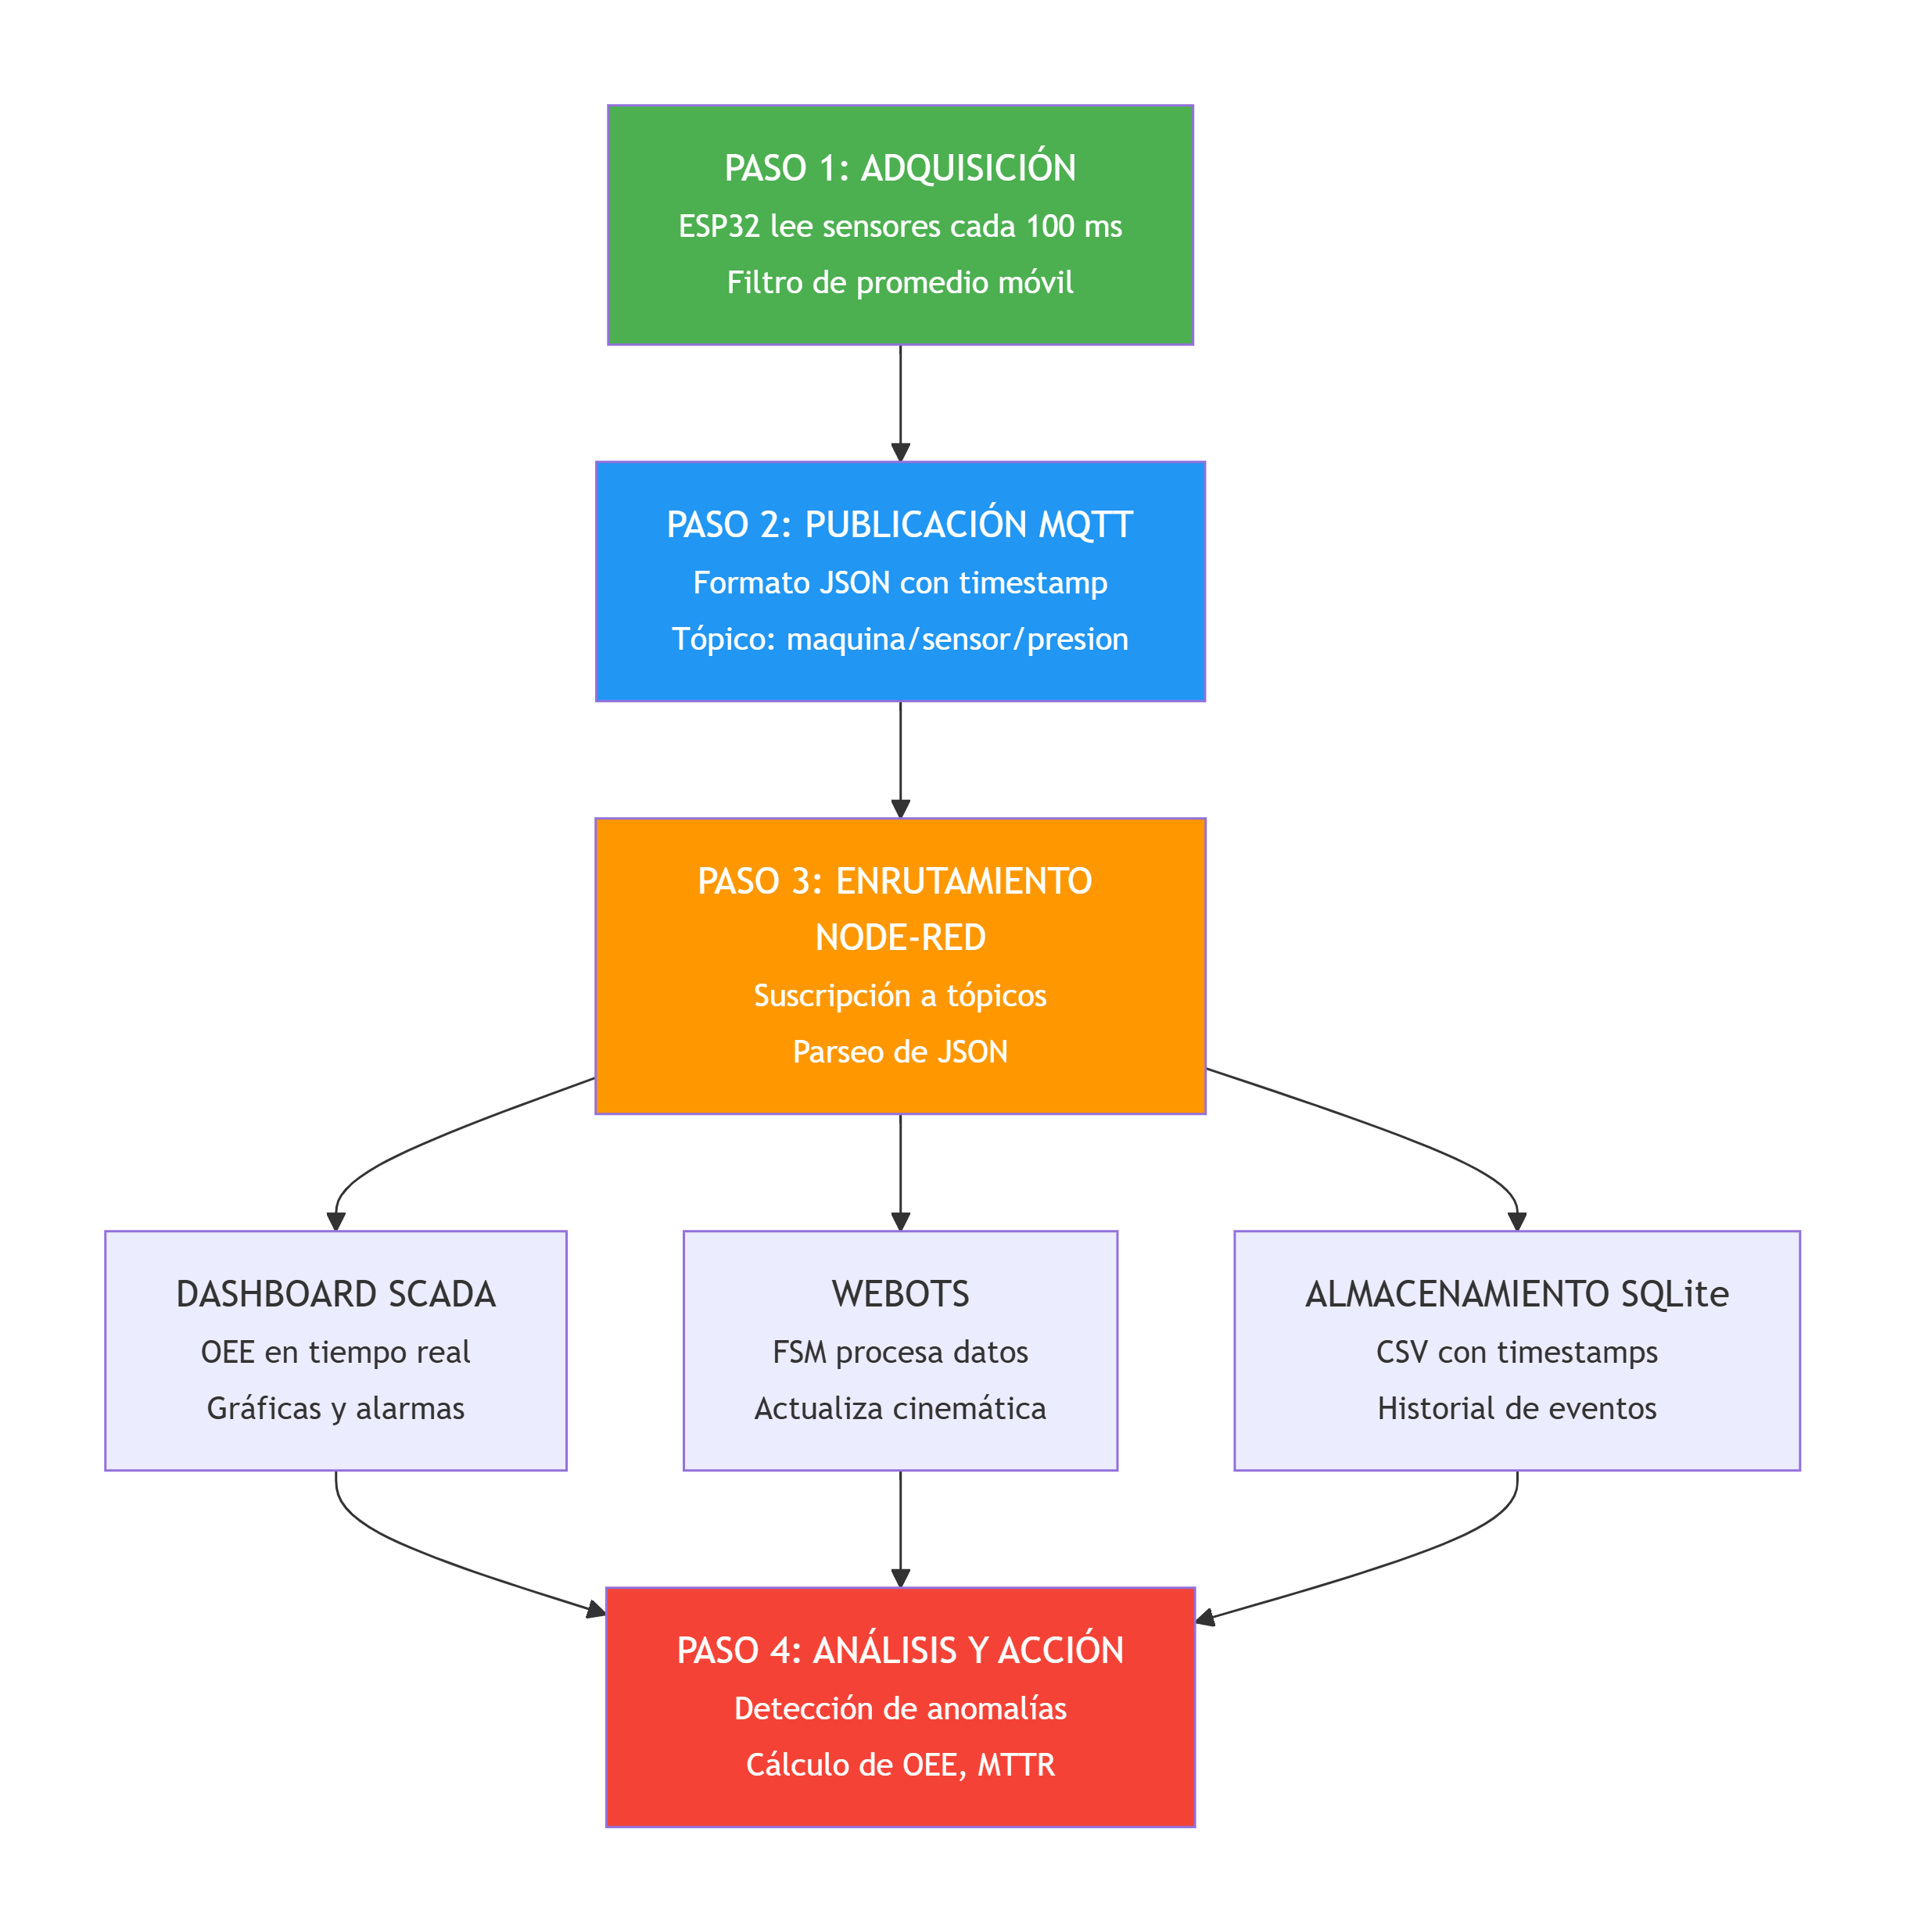
\includegraphics[width=0.9\textwidth]{Capítulos/img/ciclodevidacomunicacion.png}
\caption{Ciclo completo de la información desde el sensor hasta el registro histórico.}
\label{fig:ciclo_info}
%\end{minipage}
\end{figure}

\begin{figure}[htbp]
\centering
\begin{minipage}{0.48\textwidth}
    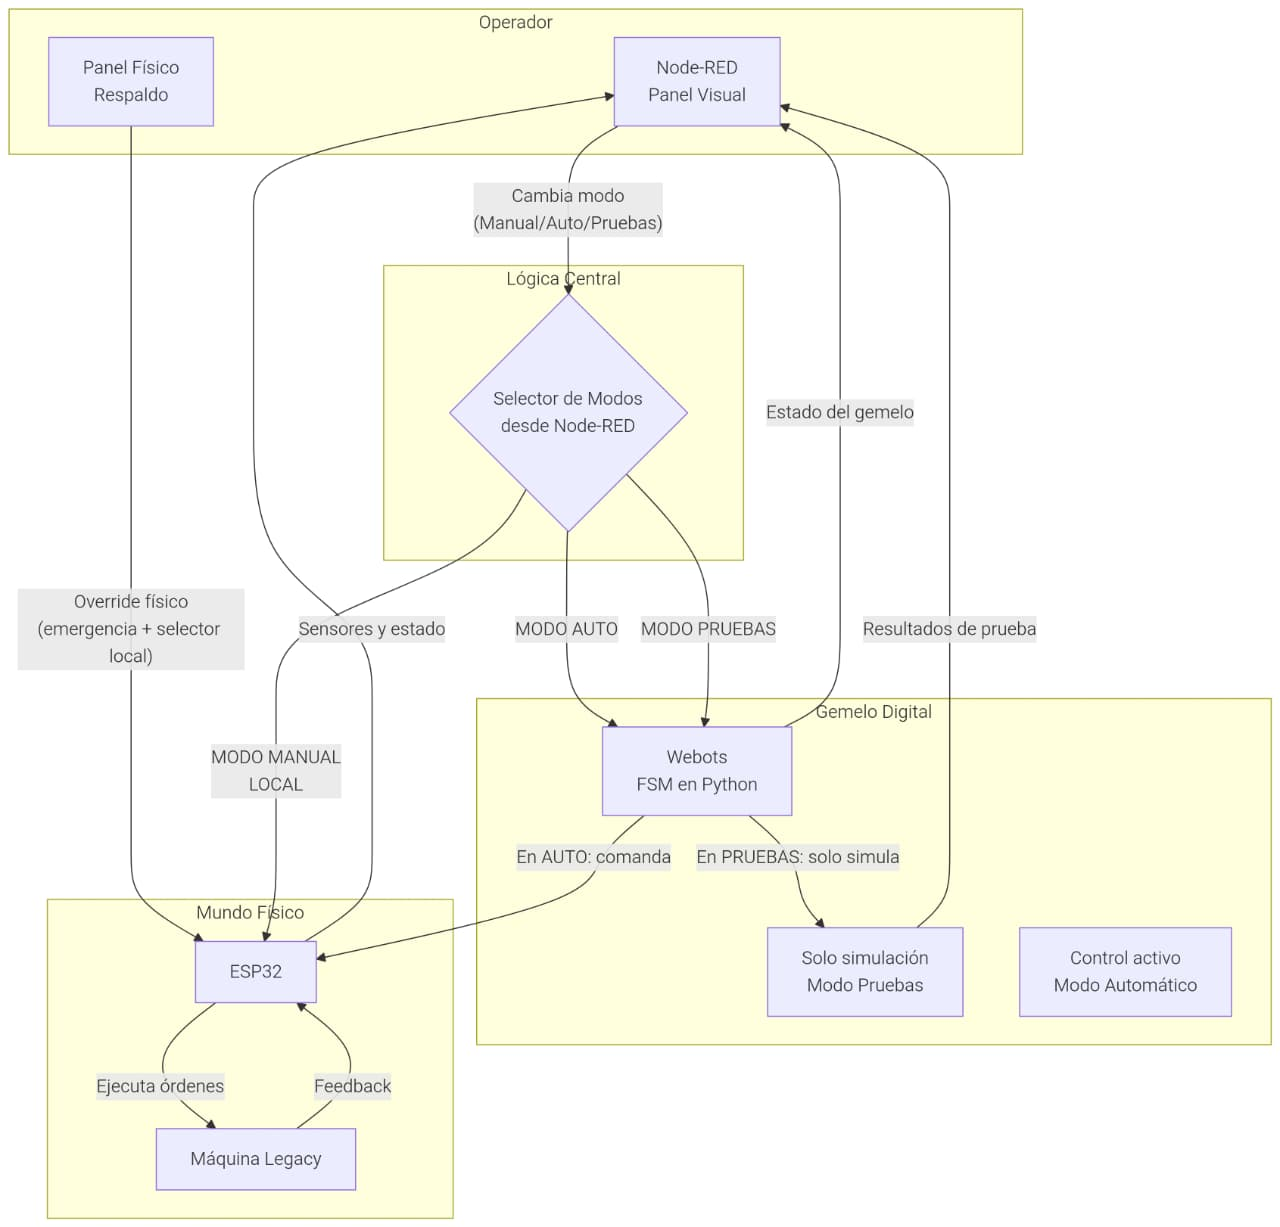
\includegraphics[width=0.9\textwidth]{Capítulos/img/arquitectura_sistema.jpeg}
\caption{Arquitectura global del gemelo digital implementado.}
\label{fig:arq_general}
\end{minipage}

\end{figure}

\subsection{Validación Geométrica del Modelo}

Para garantizar que el gemelo digital mantuviera una correspondencia volumétrica exacta, se compararon las dimensiones reales de la máquina con las del modelo importado en Webots. La Tabla~\ref{tab:comp_geom} muestra la coincidencia en distancias y posiciones de los actuadores, con una desviación máxima de 2 mm. Esta precisión es suficiente para que las restricciones cinemáticas y las colisiones se reproduzcan fielmente.

\begin{table}[htbp]
\centering
\caption{Comparación de dimensiones y posiciones geométricas.}
\label{tab:comp_geom}
\begin{tabular}{lcc}
\hline
\textbf{Parámetro} & \textbf{Valor real (mm)} & \textbf{Valor en Webots (mm)} \\
\hline
Carrera del pistón A & 80 & 80 \\
Carrera del pistón B & 120 & 120 \\
Diámetro de válvula & 35 & 35 \\
\hline
\end{tabular}
\end{table}

\section{Justificación Técnica y Adaptación de Métricas}

\subsection{Selección Tecnológica}

La elección del ESP32 frente a otras plataformas (Arduino, Raspberry Pi) se fundamenta en su conectividad WiFi integrada, su arquitectura dual-core (que permite manejar la comunicación MQTT y la lógica de control en paralelo) y su bajo costo, convirtiéndolo en la opción idónea para el nodo de borde del sistema ciberfísico \cite{espressif2023}. MQTT fue seleccionado sobre HTTP por su menor sobrecarga de cabeceras, su modelo de publicación/suscripción asíncrono y su amplia adopción en entornos IIoT, tal como lo respalda el estándar OASIS \cite{oasis2014}. Webots se impuso a otros simuladores (Nvidia Isaac Sim, Gazebo, Unity) por su integración nativa con Python, su bajo consumo de CPU y su capacidad para modelar restricciones mecánicas discretas sin necesidad de motores físicos complejos, características que lo consolidan como un entorno de simulación profesional para robótica y automatización \cite{michel2004}. Por último, Node-RED se prefirió a un SCADA tradicional por su entorno de programación visual, su conectividad MQTT nativa y la posibilidad de desplegar dashboards web de manera ágil, funcionalidades que han sido validadas en aplicaciones de IoT industrial.

\subsection{Adaptación de Métricas}

La métrica de referencia en la industria es la Efectividad Global del Equipo (OEE, por sus siglas en inglés), definida como el producto de la disponibilidad, el rendimiento y la calidad según la norma ISO 22400-2 \cite{iso22400-2}. La literatura especializada señala que el OEE es una herramienta clave para medir el desempeño de los equipos de manufactura \cite{muchiri2008}. Dado que en este proyecto no se dispone de celdas de carga ni de sistemas de visión artificial para medir la calidad del producto dosificado, se adaptó el OEE eliminando el factor de calidad, obteniendo así la \textbf{Efectividad Mecánica Operativa (EMO)}:

\begin{equation}
    \text{EMO} (\%) = \text{Disponibilidad} \times \text{Rendimiento} \times 100.
    \label{eq:emo}
    \addeqtolist{EMO: Efectividad Mecánica Operativa}
\end{equation}

Adicionalmente, se calculó el Tiempo Medio de Recuperación (\textit{Mean Time To Repair}, MTTR) ante fallos inyectados durante la fase de verificación:

\begin{equation}
    \text{MTTR} = \frac{\sum_{i=1}^{N} \text{tiempo de inactividad}_i}{N}.
    \label{eq:mttr}
    \addeqtolist{MTTR: Tiempo Medio de Recuperación}
\end{equation}

donde \(N\) es el número de eventos de fallo inducidos.

Los filtros de promedio móvil aplicados a la señal de presión siguen la ecuación:

\begin{equation}
    \overline{p}_k = \frac{1}{M} \sum_{i=0}^{M-1} p_{k-i}.
    \label{eq:presion}
    \addeqtolist{Filtro de promedio móvil para presión}
\end{equation}

con \(M=10\) muestras, suficiente para atenuar el ruido de conmutación del contactor sin introducir un retardo excesivo.

\section{Presupuesto y Recursos Económicos}

La inversión total necesaria para la implementación del bypass, la instrumentación y los nodos de comunicación se desglosa en la Tabla~\ref{tab:presupuesto}. Los precios corresponden a valores de mercado locales, y se incluye una partida para herramientas de laboratorio considerando una depreciación del 50\% de su vida útil.

\begin{longtable}{|p{6.5cm}|c|p{2cm}|c|}
\caption{Presupuesto detallado del proyecto.}
\label{tab:presupuesto}
\\\hline
\textbf{Componente/Herramienta} & \textbf{Cantidad} & \textbf{Precio Unitario (USD)} & \textbf{Subtotal (USD)} \\
\hline
\endfirsthead
\hline
\textbf{Componente/Herramienta} & \textbf{Cantidad} & \textbf{Precio Unitario (USD)} & \textbf{Subtotal (USD)} \\
\hline
\endhead
\hline
\endlastfoot
ESP32 DevKit v1 (38 pines) & 2 & 6.50 & 13.00 \\
Optoacopladores PC817 & 10 & 0.30 & 3.00 \\
Sensor de presión industrial 4-20 mA & 1 & 65.00 & 65.00 \\
Válvula reguladora de presión & 1 & 45.00 & 45.00 \\
Módulo relé 8 canales 5 V/10 A & 1 & 8.50 & 8.50 \\
Fuente switching 12 V/10 A & 1 & 22.00 & 22.00 \\
Módulo Buck XL4015 & 1 & 3.50 & 3.50 \\
Display TM1637 & 1 & 2.80 & 2.80 \\
Caja electrónica IP54 & 1 & 18.00 & 18.00 \\
Selector 3 posiciones & 1 & 4.00 & 4.00 \\
Botones pulsadores industriales & 12 & 1.20 & 14.40 \\
Cables jumper, AWG, conectores & Global & 15.00 & 15.00 \\
Kit de soldadura y herramientas & Global & 30.00 & 30.00 \\
\hline
\textbf{TOTAL} & & & \textbf{243.20} \\
\hline
\end{longtable}